\documentclass[12pt,letterpaper]{article}

\usepackage[margin=0.85in]{geometry}
\usepackage[T1]{fontenc}
\usepackage{lmodern}
\usepackage[scaled=0.95]{helvet}
\renewcommand{\familydefault}{\sfdefault}
\usepackage{amsmath}
\usepackage{array}
\usepackage{tabularx}
\usepackage[table]{xcolor}
\usepackage{tikz}
\usetikzlibrary{arrows.meta}
\usepackage[most]{tcolorbox}
\usepackage{titlesec}
\usepackage{fancyhdr}
\usepackage{needspace}

% ---------- Colors ----------
\definecolor{monster}{HTML}{1F6FB5}   % Cookie Monster blue
\definecolor{cookiedark}{HTML}{7A4A22}
\definecolor{grover}{HTML}{2E6DB4}
\definecolor{count}{HTML}{6B3FA0}     % The Count purple
\definecolor{elmo}{HTML}{D32F2F}
\definecolor{cookie}{HTML}{C68B4E}
\definecolor{chip}{HTML}{3B2314}
\definecolor{softyellow}{HTML}{FFF6DD}
\definecolor{softblue}{HTML}{E8F1FA}
\definecolor{softpurple}{HTML}{F1EBF8}
\definecolor{gold}{HTML}{C68B4E}

% ---------- Headings ----------
\titleformat{\section}{\Large\bfseries\color{cookiedark}}{}{0pt}{}
\titlespacing*{\section}{0pt}{14pt}{6pt}
\setcounter{secnumdepth}{0}

\pagestyle{fancy}
\fancyhf{}
\renewcommand{\headrulewidth}{0pt}
\fancyfoot[C]{\small\color{gray}Cookie Monster's Growing Cookie Jar \textperiodcentered\ page \thepage}

\setlength{\parindent}{0pt}
\setlength{\parskip}{6pt}

% ---------- Helpers ----------
% A cookie with chocolate chips
\newcommand{\cookie}[1][1]{%
  \begin{tikzpicture}[scale=#1, baseline=-0.6ex]
    \fill[cookie] (0,0) circle (0.5);
    \draw[cookiedark, line width=0.8pt] (0,0) circle (0.5);
    \foreach \x/\y in {-0.2/0.2, 0.15/0.25, 0.25/-0.1, -0.1/-0.25, -0.28/-0.05, 0.05/0.0}
      \fill[chip] (\x,\y) circle (0.06);
  \end{tikzpicture}}

% A cookie jar filled to fraction #2 (0 to 1), drawn at (#1,0)
\newcommand{\jar}[2]{%
  \fill[cookie!70] (#1-0.7,0) rectangle (#1+0.7,{1.8*#2});
  \draw[cookiedark, line width=1.2pt, rounded corners=4pt]
    (#1-0.7,1.8) -- (#1-0.7,0) -- (#1+0.7,0) -- (#1+0.7,1.8);
  \draw[cookiedark, line width=1.2pt, fill=cookiedark!30] (#1-0.8,1.8) rectangle (#1+0.8,2.05);}

\newcommand{\blank}[1][3cm]{\underline{\hspace{#1}}}

\newcounter{question}
\newcommand{\question}{%
  \refstepcounter{question}\par\needspace{3\baselineskip}%
  \textbf{\color{monster}Question \arabic{question}.}~}

\newtcolorbox{bigidea}[1][]{enhanced, colback=softyellow, colframe=gold,
  boxrule=1pt, arc=3mm, left=8pt, right=8pt, top=6pt, bottom=6pt, #1}
\newtcolorbox{tryit}{enhanced, colback=softblue, colframe=monster,
  boxrule=0.8pt, arc=3mm, left=8pt, right=8pt}
\newtcolorbox{mathclub}[1]{enhanced, colback=softpurple, colframe=count,
  boxrule=0.8pt, arc=3mm, left=8pt, right=8pt, top=4pt, bottom=4pt,
  title={\textbf{#1}}, colbacktitle=count, coltitle=white}

\renewcommand{\arraystretch}{1.6}

\begin{document}

% ================= Title =================
\begin{center}
  {\cookie[0.9]\hspace{0.6em}\cookie[0.9]\hspace{0.6em}\cookie[0.9]}\\[6pt]
  {\Huge\bfseries\color{cookiedark} Cookie Monster's Growing Cookie Jar}\\[4pt]
  {\Large Where the Number $e$ Comes From}\\[6pt]
  {\small\color{gray} November 4, 2026 \textperiodcentered\ Nathaniel}
\end{center}

\vspace{2pt}
Name: \blank[6cm] \hfill Date: \blank[4cm]

% ================= The story =================
\section{The story}

\textbf{\color{monster}Cookie Monster} has a \textbf{magic cookie jar}. It starts with
\textbf{256 cookies}. Once a day, the jar \textbf{grows}: it makes as many new cookies as it
already has. But only if Cookie Monster does not eat any! \emph{``Me wait. Me wait. Me
VERY hungry, but me wait!''}

Then \textbf{\color{grover}Grover} has an idea: \emph{``What if the jar grows a LITTLE bit,
MANY times a day? Would that make MORE cookies?''} Let's find out. We will discover a famous
number called $\boldsymbol{e}$.

% ================= One step =================
\section{Growing once}

Once a day, the jar adds as many cookies as it has. That means it \textbf{doubles}.

\question The jar has 256 cookies. It adds 256 more. \quad $256 + 256 = $ \blank[2cm]

\begin{center}
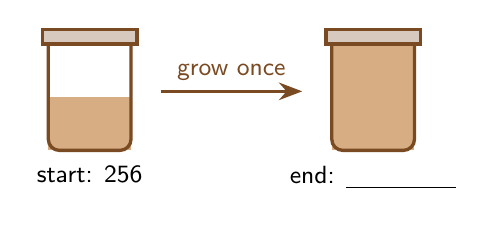
\begin{tikzpicture}[scale=0.75, every node/.style={transform shape=false}]
  \jar{0}{0.5}
  \node[below, font=\small] at (0,-0.1) {start: 256};
  \draw[-{Stealth}, line width=1.2pt, cookiedark] (1.2,1) -- (3.6,1)
    node[midway, above, font=\small] {grow once};
  \jar{4.8}{1}
  \node[below, font=\small] at (4.8,-0.1) {end: \blank[1.4cm]};
\end{tikzpicture}
\end{center}

% ================= Two steps =================
\section{Grover's idea: grow two times, a half each time}

\emph{``Grow \textbf{two} times a day, but each time add only \textbf{half} of what is in the
jar!''} Remember: a half is one of two equal parts.

\question Fill in the table. The first row is done for you.

\begin{center}
\renewcommand{\arraystretch}{1.45}
\rowcolors{2}{white}{softyellow}
\begin{tabular}{|>{\centering\arraybackslash}p{2.4cm}|>{\centering\arraybackslash}p{3.4cm}|>{\centering\arraybackslash}p{3.4cm}|>{\centering\arraybackslash}p{3.4cm}|}
\hline
\rowcolor{cookiedark}
\textbf{\color{white}Grow} & \textbf{\color{white}Cookies in jar} & \textbf{\color{white}Add half} & \textbf{\color{white}New total} \\
\hline
1st time & 256 & 128 & 384 \\ \hline
2nd time & 384 &     &     \\ \hline
\end{tabular}
\end{center}

\question Two halves made \blank[2cm] cookies. Is that \textbf{more} than growing once
(Question~1)? \blank[2cm]

% ================= Four steps =================
\newpage
\section{Grow four times, a quarter each time}

\emph{``Even MORE times! Grow \textbf{four} times, and each time add a \textbf{quarter}!''}

\begin{tryit}
\textbf{Quarter trick:} a quarter is \textbf{half of a half}. To find a quarter of 256, take half
(128), then half again (64). So a quarter of 256 is 64.
\end{tryit}

\question Use the quarter trick to fill in the table.

\begin{center}
\renewcommand{\arraystretch}{1.45}
\rowcolors{2}{white}{softyellow}
\begin{tabular}{|>{\centering\arraybackslash}p{2.4cm}|>{\centering\arraybackslash}p{3.4cm}|>{\centering\arraybackslash}p{3.4cm}|>{\centering\arraybackslash}p{3.4cm}|}
\hline
\rowcolor{cookiedark}
\textbf{\color{white}Grow} & \textbf{\color{white}Cookies in jar} & \textbf{\color{white}Add a quarter} & \textbf{\color{white}New total} \\
\hline
1st time & 256 & 64  & 320 \\ \hline
2nd time & 320 &     &     \\ \hline
3rd time &     &     &     \\ \hline
4th time &     &     &     \\ \hline
\end{tabular}
\end{center}

\question Fill in what The Count found so far.
\emph{``Ah ah ah! Let me count the cookies!''}

\begin{center}
\renewcommand{\arraystretch}{1.45}
\begin{tabular}{|>{\centering\arraybackslash}p{4.2cm}|>{\centering\arraybackslash}p{3.6cm}|}
\hline
\rowcolor{count}
\textbf{\color{white}How the jar grows} & \textbf{\color{white}Cookies at the end} \\ \hline
1 time, add all of it & \\ \hline
2 times, add a half & \\ \hline
4 times, add a quarter & \\ \hline
\end{tabular}
\end{center}

\question More, smaller steps made \blank[2.5cm] cookies. (more or fewer?)

% ================= Many steps =================
\section{What if we grow MANY times?}

The steps get too tiny to do by hand, so The Count used a computer. Here is what he found:

\begin{center}
\renewcommand{\arraystretch}{1.35}
\rowcolors{2}{white}{softpurple}
\begin{tabular}{|>{\centering\arraybackslash}p{5.6cm}|>{\centering\arraybackslash}p{3.6cm}|}
\hline
\rowcolor{count}
\textbf{\color{white}How many tiny steps in a day} & \textbf{\color{white}Cookies at the end} \\ \hline
8 & about 657 \\ \hline
100 & about 692 \\ \hline
1,000 & about 696 \\ \hline
1,000,000 (one million!) & about 696 \\ \hline
\end{tabular}
\end{center}

\question Does the jar keep growing bigger and bigger forever, or does it stop near one
number? \blank[3cm]

\begin{bigidea}
More steps make more cookies, but not forever! The jar gets closer and closer to
\textbf{about 696 cookies}, and never goes past it. Grover's idea helps, but only up to a point.
\end{bigidea}

% ================= Jars =================
\newpage
\section{How many jars full?}

The jar started with 256 cookies. Call that \textbf{one jarful}. How many jarfuls is 696 cookies?

\begin{center}
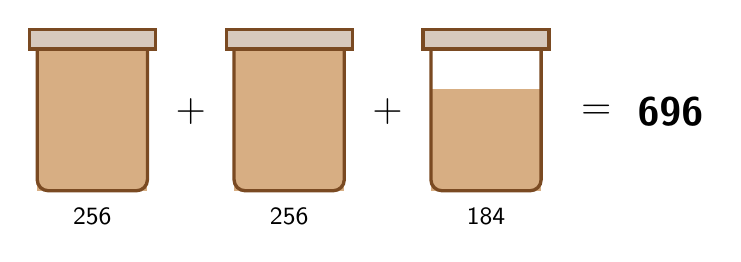
\begin{tikzpicture}
  \jar{0}{1}   \node[below, font=\small] at (0,-0.1) {256};
  \node[font=\Large] at (1.25,1) {$+$};
  \jar{2.5}{1} \node[below, font=\small] at (2.5,-0.1) {256};
  \node[font=\Large] at (3.75,1) {$+$};
  \jar{5}{0.72} \node[below, font=\small] at (5,-0.1) {184};
  \node[font=\Large] at (6.4,1) {$=$};
  \node[font=\Large\bfseries, anchor=west] at (6.8,1) {696};
\end{tikzpicture}
\end{center}

\question Two full jars is $256 + 256 = $ \blank[1.6cm] cookies. The last jar is a little less
than \blank[1.6cm] full. (half or three-quarters?)

\begin{bigidea}
That is \textbf{2 jarfuls and a bit more than 7 tenths of another}: about
$\boldsymbol{2.72}$ jarfuls. Mathematicians call this number $\boldsymbol{e}$:
\[
  e \approx 2.72
\]
It is the number you get when something \textbf{grows in tiny, tiny steps}. The jar ends with
$e$ jarfuls, no matter how many cookies it starts with!
\end{bigidea}

\question A different magic jar starts with 100 cookies. About how many cookies
will it have after growing in tiny steps? (Hint: $e$ jarfuls of 100.) \quad about \blank[1.8cm]

\begin{mathclub}{The Count's Math Club: write it like a scientist}
The number $e$ is named after \textbf{Leonhard Euler} (say ``OY-ler''), who studied it. It goes
on forever without repeating: $e = 2.71828\ldots$ Scientists write ``grow by all of it, in
$n$ tiny steps'' like this:
\[
  \left(1 + \frac{1}{n}\right)^{n} \;\longrightarrow\; e \quad\text{when $n$ gets very big.}
\]
The little $n$ up high means ``do it $n$ times.'' With $n = 4$ you did
$\left(1 + \frac{1}{4}\right)^4$: add a quarter, four times!
\end{mathclub}

\begin{tcolorbox}[enhanced, colback=softblue, colframe=elmo, boxrule=1pt, arc=3mm,
  title={\textbf{Coming up: The Cookie Circle}}, colbacktitle=elmo, coltitle=white]
Here is Euler's big surprise. If the jar grows in tiny steps, you get $e$. But if each tiny
step is a tiny \textbf{turn}, using $j$ from The Count's Square Cookies, you do not grow at
all. You walk around a \textbf{circle}! That is why $e$ and $j$ meet in Euler's famous
equation, $e^{j\pi} + 1 = 0$.
\end{tcolorbox}

{\small\color{gray}\textbf{For teachers:} this is compound growth at a 100\% rate:
$256\,(1 + 1/n)^n$ gives 512, 576 and 625 for $n = 1, 2, 4$, and tends to $256\,e \approx 695.9$
(the table values are rounded). The 256-cookie start keeps every hand-computed step a whole
number. The ``Coming up'' box previews $e^{j\theta} = \lim_{n\to\infty}(1 + j\theta/n)^n$: each
factor $1 + j\theta/n$ is, to first order, a rotation by $\theta/n$, so the product rotates by
$\theta$. Sesame Street characters appear by name only, for classroom use; this worksheet is not
affiliated with or endorsed by Sesame Workshop.}

% ================= Answer key =================
\newpage
\section{Answer key}

\begin{center}
\rowcolors{2}{white}{softyellow}
\begin{tabularx}{\linewidth}{|>{\centering\arraybackslash}p{2.8cm}|X|}
\hline
\rowcolor{cookiedark}
\textbf{\color{white}Question} & \textbf{\color{white}Answer} \\ \hline
1 & 512 \\ \hline
2 & 2nd time: 384, add 192, total 576 \\ \hline
3 & 576; yes, more than 512 \\ \hline
4 &
  \begin{tabular}[t]{@{}llll@{}}
    2nd: & 320, & add 80, & total 400 \\
    3rd: & 400, & add 100, & total 500 \\
    4th: & 500, & add 125, & total 625
  \end{tabular} \\ \hline
5 & 512; 576; 625 \\ \hline
6 & More \\ \hline
7 & It stops near one number (about 696) \\ \hline
8 & 512; three-quarters (184 out of 256 is about 0.72) \\ \hline
9 & About 272 (2.72 jarfuls of 100) \\ \hline
\end{tabularx}
\end{center}

\end{document}
